\documentclass[a4paper,12pt]{article} 
\usepackage[T2A]{fontenc}			
\usepackage[utf8]{inputenc}			
\usepackage[english,russian]{babel}	
\usepackage{amsmath,amsfonts,amssymb,amsthm,mathtools} 
\usepackage[colorlinks, linkcolor = blue]{hyperref}
\usepackage{upgreek}
\usepackage[left=2cm,right=2cm,top=2cm,bottom=3cm,bindingoffset=0cm]{geometry}
\usepackage{multirow}
\usepackage{graphicx}
\usepackage{xcolor}
\usepackage{multirow}
\usepackage{pgfplots}
\usepackage{pgfplotstable}
\pgfplotsset{compat=1.9}

\pgfplotstableset{ %
        create on use/SquareLight/.style={
                create col/expr={\thisrow{Dark}}}
}

\author{Шелихов Дмитрий\\Группа Б01-305}

\title{\textbf{Работа 3.2.5\\Свободные и вынужденные колебания в электрическом контуре}} 
\date{\today}

\begin{document} 
\maketitle

\textbf{Цель работы:} Исследование свободных и вынужденных колебаний в колебательном контуре. \\

\textbf{В работе используются: } Осциллограф АКТАКОМ ADS-6142H, генератор сигналов специальной формы АКИП-3409/4, магазин сопротивления МСР-60, магазин емкости Р5025, магазин индуктивности Р567 типа МИСП, соединительная коробка с шунтирующей емкостью, соединительные одножильные и коаксиальные провода. \\

\textbf{Экспериментальная установка: }

\par Схема установки для исследования колебаний приведена на рисунке 1.
Колебательный контур состоит из постоянной индуктивности L с активным сопротивлением $R_L$, переменной емкости C и сопротивления R. Картина колебаний
напряжения на емкости наблюдается на экране двухканального осциллографа.

\par Сигнал с генератора поступает через конденсатор $C_1$ на вход колебательного контура. Данная ёмкость необходима, чтобы выходной импеданс генератора был много меньше импеданса колебательного контура и не влиял на процессы, проходящие в контуре. 

\par При изучении свободно затухающих колебаний, генератор специальных сигналов на вход колебательного контура подает периодические короткие импульсы, которые заряжают конденсатор C. За время между последовательными импульсами происходит разрядка конденсатора через резистор и катушку индуктивности. $U_C$ подается на канал 1(X) осциллографа. Для наблюдения фазовой картины затухающих колебаний на канал 2(Y) подается напряжение с резистора R, которое пропорционально току I.

\par При изучении возбужденных колебаний на вход колебательного контура подается синусоидальный сигнал. С помощью осциллографа возможно измерить зависимость амплитуды возбужденных колебаний в зависимости от частоты внешнего сигнала, из которого возможно определить добротность колебательного контура. Альтернативным способом расчета добротности контура является определение декремента затухания по картине установления возбужденных колебаний. В этом случае генератор сигналов используется для подачи цугов синусоидальной формы.

\begin{figure}
\center{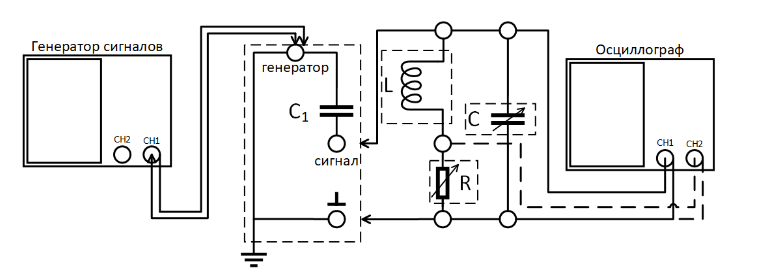
\includegraphics[width=.8\textwidth]{1.png}}
\caption{Схема установки для исследования вынужденных колебаний}
\end{figure}

\textbf{Ход работы}
\textbf{Подготовка приборов к работе}

\par 1) Подключим генератор специальных сигналов к входу 1(X) осциллографа. \\
\par 2) Установим на генераторе специальных сигналов последовательность импульсов. Установим длительность импульсов 10 мкс, частоту повторения импульсов $\nu$ = 100 Гц, а амплитуду сигнала 20 В. Подадим сигнал.\\
\par 3) Видим, что на осциллографе отображаются периодические импульсы. Получим статичное изображние с помощью настройки синхронизации. \\
\par 4) Соберем схему согласно рис.1.

\textbf{Измерение периодов свободных колебаний}

\par 1) Установим на магазине сопротивлений величину R = 0 Ом, на магазине индуктивностей L = 100 мГн, на магазине ёмкостей C = 0 мкФ. Контур сам по себе обладает некоторым минимальным значением емкости $C_0$, благодаря которому в контуре реализуются свободные колебания. При этом затухание обеспечивается наличием активного сопротивления в магазине индуктивностей $R_L$. Получим на экране картину свободных затухающих колебаний с помощью настроек осциллографа. На экране осциллографа появился сигнал, который соответствует свободным колебаниям с затуханием. \\ 

\par 2) Подберём частоту развертки осциллографа при котором расстояние между импульсами генератора занимает почти весь экран. \\
\par 3) Измерим с помощью осциллографа период затухающих колебаний:\\

\begin{center}
\begin{tabular}{|c|c|}
	\hline
	T, мкс & 70 $\pm$ 1 \\
	\hline
\end{tabular}
\end{center}

\par 4) По периоду колебаний определим нулевую ёмкость ($C_0$) колебательного контура. Это значение является минимальным для магазина ёмкостей и его необходимо учитывать (прибавлять) при дальнейших расчётах. 

\begin{center}
\begin{tabular}{|c|c|}
	\hline
	$C_0$, нФ & 1.24 $\pm$ 0.04\\
	\hline
\end{tabular}
\end{center}

\par 5) Изменяя ёмкость от 0 мкФ до 0.009 мкФ проведем измерения периодов. Рассчитаем теоретические значения по формуле $T = 2\pi\sqrt{LC}$.

\begin{center}
\begin{tabular}{|c|c|c|c|}
	\hline
	C, мкФ & $T_{\text{эксп}}$, мкс & $T_{\text{теор}}$, мкс & L, мГн \\
	\hline 
	0,001 & 95 $\pm$ 1 & 94,04 $\pm$ 0,14 & \multirow{9}{*}{100,0 $\pm$ 0,2} \\
	\cline {1-3}  0,002 & 114 $\pm$ 2 & 108,83 $\pm$ 0,16 & \\
	\cline {1-3}  0,003 & 130 $\pm$ 2 & 140,50 $\pm$ 0,21 & \\
	\cline {1-3}  0,004 & 144 $\pm$ 2 & 166,24 $\pm$ 0,25 & \\
	\cline {1-3}  0,005 & 159 $\pm$ 2 & 188,50 $\pm$ 0,28 & \\
	\cline {1-3}  0,006 & 170 $\pm$ 3 & 208,39 $\pm$ 0,21 & \\
	\cline {1-3}  0,007 & 182 $\pm$ 3 & 226,54 $\pm$ 0,34 & \\
	\cline {1-3}  0,008 & 187 $\pm$ 3 & 243,35 $\pm$ 0,37 & \\
	\cline {1-3}  0,009 & 199 $\pm$ 3 & 259,06 $\pm$ 0,39 & \\
	\hline	
\end{tabular}
\end{center}

\par Построим график $T_{\text{эксп}}$ = f($T_{\text{теор}}$): 

\pgfplotstableread{
x	y 		y-max 	y-min
94.04	95	1	1
108.83	114	2	2
140.50	130	2	2
166.24	144	2	2
188.50	159	2	2
208.39	170	3	3
226.54	182	3	3
243.55	187	3	3
259.06	199	3	3
}{\mytable}

\begin{center}
\begin{tikzpicture}
\begin{axis} [
	title = $T_{\text{эксп}} f(T_{\text{теор}})$,
	xlabel = {$T_{\text{теор}}$, мкс},
	ylabel = {$T_{\text{эксп}}$, мкс},
	minor tick num = 2,
	grid = major
]

\addplot +[mark options = {scale = 0.1,}]
	plot [error bars/.cd, y dir=both, y explicit]
	table [y error plus=y-max, y error minus=y-min] {\mytable};

\addplot +[mark options = {scale = 0,}]
	table[row sep=\\,				%аппроксимация
   y={create col/linear regression={y=Y}}]
    {
   		X Y\\  
		94.04          95\\
	 	108.83         114\\
	 	140.50         130\\
	 	166.24         144\\
	 	188.50         159\\
	    208.39         170\\
	 	226.54         182\\
 	 	243.55         187\\
	 	259.06         199\\ 
    };
	\addlegendentry{
        k$\approx \pgfmathprintnumber{\pgfplotstableregressiona}$} 

\end{axis}
\end{tikzpicture}
\end{center}

Откуда получаем зависимость, которая аппроксимируется прямой $T_{\text{эксп}} \approx 0.6 T_{\text{теор}}$. 

\par Теоретические значения отклоняются от экспериментальных при увеличении ёмкости из-за наличия сопротивления обкладок конденсатора, которое возрастает при увеличении ёмкости. 

\par\textbf{Критическое сопротивление и декремент затухания} 

\par 1) Приняв L = 100 мГн, рассчитаем ёмкость $C^*$, при которой собственная частота колебаний $\nu_0$ = $\frac{1}{2\pi\sqrt{LC}}$ = 6.5 кГц. Для выбранных L и $C^*$ рассчитаем критическое сопротивление контура $R_{\text{cr}}$ по формуле $R_{\text{cr}} = 2\sqrt{L/{C^*}}$

\begin{center}
\begin{tabular}{|c|c|c|c|}
	\hline
	$C^*$, нФ & L, мГн & $\nu_0$, кГц & $R_{\text{cr}}$, кОм \\
	\hline
	6.00  $\pm$ 0.01 & 100 & 6.5 & 8.165 $\pm$ 0.015 \\
	\hline
\end{tabular}
\end{center}

\par 2) Установим на магазине ёмкость, близкую к рассчитанной критической: C = 6 нФ (включая $C_0$). Увеличивая сопротивление R от нуля до $R_{\text{cr}}$, пронаблюдаем картину затухающих колебаний на экране осциллографа. Определим сопротивление магазина, при котором колебательный режим переходит в апериодический: R $\approx$ 8300 Ом. 

\par 3) Установим сопротивление R $\approx$ 0.05$R_{\text{cr}}$ = (408.25 $\pm$ 0.83) Ом. Получим на экране картину затухающих колебаний. Для расчёта логарифмического декремента затухания $\theta = \frac{1}{n}ln\frac{U_m}{U_{m+n}}$ измерим амплитуды, разделенные целым числом периодов n. Измерения проведем для 6 значений R в интервале (0.05-0.25)$R_{\text{cr}}$. 

\begin{center}
\begin{tabular}{|c|c|c|c|c|c|}
	\hline
	R, Ом & $U_m$, мВ & n & $U_{m+n}$, мВ & $\theta$ & $R_{\Sigma}$, Ом\\
	\hline
	408.25 $\pm$ 0.75 & 688 $\pm$ 7 & 3 & 224 $\pm$ 2 & 0.374 $\pm$ 0.036 & 440.58 $\pm$ 0.75 \\
	\hline
	816.50 $\pm$ 1.50 & 552 $\pm$ 6 & 3 & 80 $\pm$ 1 & 0.644 $\pm$ 0.048 & 848.83 $\pm$ 1.50\\
	\hline
	1224.75 $\pm$ 2.25 & 440 $\pm$ 4 & 3 & 30 $\pm$ 1 & 0.895 $\pm$ 0.073 & 1257.08 $\pm$ 2.25\\
	\hline
	1633.00 $\pm$ 3.00 & 348 $\pm$ 3 & 2 & 28 $\pm$ 1 & 1.260 $\pm$ 0.099 & 1665.33 $\pm$ 3.00\\
	\hline
	2041.25 $\pm$ 3.75 & 284 $\pm$ 3 & 1 & 55 $\pm$ 1 & 1.642 $\pm$ 0.126 & 2073.58 $\pm$ 3.75\\
	\hline
	2449.50 $\pm$ 4.50 & 218 $\pm$ 1 & 1 & 29 $\pm$ 1 & 2.017 $\pm$ 0.149 & 2481.83 $\pm$ 4.50\\
	\hline
\end{tabular}
\end{center}

\par Построим график в координатах 1/$\theta^2$  = f[1/($R_{\Sigma}^2$)]. Y = 1/$\theta^2$, 1/($R_{\Sigma}^2$) = X. Тогда $R_{\text{cr}} = 2\pi\sqrt{\Delta Y/\Delta X}$.

\pgfplotstableread{
x			y 			x-max		x-min				y-max 		y-min
5.1517		7.14737		0.0175		0.0175				1.39		1.39
1.3879		2.41236		0.0049		0.0049			 	0.3569		0.3569
0.63281		1.24786		0.002265	0.002265			0.203		0.203
0.360578	0.62988		0.001299	0.001299			0.0986		0.0986
0.232573	0.37105		0.0008411	0.0008411			0.05688		0.05688
0.162351	0.245755	0.000588709	0.000588709			0.05688		0.05688
}{\mytable}

\begin{center}
\begin{tikzpicture}
\begin{axis} [
	title = $X(Y)$,
	xlabel = {$X$, кОм},
	ylabel = {$Y$},
	minor tick num = 2,
	grid = major
]

\addplot +[mark options = {scale = 0.1,}]
	plot [error bars/.cd, y dir=both, y explicit]
	table [y error plus=y-max, y error minus=y-min, x error plus=x-max, x error minus=x-min] {\mytable};

\addplot +[mark options = {scale = 0,}]
	table[row sep=\\,				%аппроксимация
   y={create col/linear regression={y=Y}}]
    {
   		X Y\\ 
   		1.3879		   2.41236\\
	 	0.63281        1.24786\\
	 	0.360578       0.62988\\
	 	0.232573       0.37105\\
	 	0.162351       0.245755\\
    };
	\addlegendentry{
        k$\approx \pgfmathprintnumber{\pgfplotstableregressiona}$} 
\end{axis}
\end{tikzpicture}
\end{center}

\par Получили k = 1.77 $\pm$ 0.07: 

\begin{center}
\begin{tabular}{|c|c|}
	\hline
	$R_{\text{cr}^{\text{теор}}}$, кОм & $R_{\text{cr}^{\text{эксп}}}$, кОм \\
	\hline
	8.165 $\pm$ 0.015 & 8.359 $\pm$ 0.585\\
	\hline
\end{tabular}
\end{center}

\par Рассчитаем добротность контура Q = $\frac{\pi}{\theta}$ для максимального и минимального значений $\theta$ по картине затухающих колебаний. 

\begin{center}
\begin{tabular}{|c|c|}
	\hline
	$\theta_{\text{min}}$ = 0.374 $\pm$ 0.036 & Q = 8.4 $\pm$ 0.8 \\
	\hline
	$\theta_{\text{max}}$ = 2.017 $\pm$ 0.149 & Q = 1.6 $\pm$ 0.1 \\
	\hline
\end{tabular}
\end{center}

\par 4) Выберем R1 = (816.50 $\pm$ 1.50) Ом и R2 = (1633.00 $\pm$ 3.00) Ом. Эти значения будем использовать для наблюдения вынужденных колебаний. 

\par \textbf{Свободные колебания на фазовой плоскости}

\par 1) Введем сопротивление R $\approx$ 0.05 $R_{\text{cr}}$ на магазине. Подадим на канал 2(Y) осциллографа падение напряжения с резистора. \\

\par 2) Для одновременного наблюдения осциллограмм тока и напряжения свободных затухающих колебаний переведем осциллограф в двухканальный режим. Подберем масштабы по вертикали и частоту развертки по горизонтали так, чтобы оба сигнала были представлены на временном интервале, слегка превышающем период повторения импульсов с генератора. \\

\par 3) Подберем частоту повторения импульсов на генераторе так, чтобы расстояние между импульсами было порядка характерного времени затухания свободных колебаний. (400-500 Гц) \\

\par 4) Настроим спираль в фазовой плоскости подобрав масштаб, удобный для измерений. \\

\par Для определения декремента затухания $\theta$ измерим координаты пересечения витков спирали с горизонтальной осью координат, разделенные целым числом периодов n, для сопротивлений $R_1$ и $R_2$\\ 

$$ \theta = ln\frac{X_k}{X_{\text{k+1}}} $$

\begin{center}
\begin{tabular}{|c|c|c|c|}
	\hline
	R, Ом & i & $X_i$, усл.ед. & $\theta$ \\
	\hline
	\multirow{6}{*}{816.50 $\pm$ 1.59} & 0 & -39 & \\
	\cline{2-4} & 1 & -19 & 0.72 \\
	\cline{2-4} & 2 & -10 & 0.64 \\
	\cline{2-4} & 3 & 7 &  \\
	\cline{2-4} & 4 & 14 & 0.69 \\
	\cline{2-4} & 5 & 28 & 0.69 \\
	\hline
	\multirow{5}{*}{1633.00 $\pm$ 3.00} & 0 & -34 & \\
	\cline{2-4} & 1 & -8 & 1.45 \\
	\cline{2-4} & 2 & -2 & 1.39 \\
	\cline{2-4} & 4 & 4 & \\
	\cline{2-4} & 17 & 1.45 \\
	\hline
\end{tabular}
\end{center}

\par Откуда находим $\theta$ для обоих случаев и добротность контура Q:

\begin{center}
\begin{tabular}{|c|c|c|}
	\hline
	R, Ом & $\theta$ & Q \\
	\hline
	816.50 $\pm$ 1.59 & 0.69 $\pm$ 0.02 & 4.55 $\pm$ 0.13 \\
	\hline
	1633.00 $\pm$ 3.00 & 1.43 $\pm$ 0.03 & 2.20 $\pm$ 0.05 \\
	\hline
\end{tabular} 
\end{center}

\par\textbf{Теоретические значения для Q по R, L, C контура} 

\begin{center}
\begin{tabular}{|c|c|c|c|}
	\hline
	L, мГн & C, нФ & R, Ом & Q \\
	\hline
	99.96 & 6 & 848.83 & 4.81 \\
	\hline
	99.96 & 6 & 1665.33 & 2.45\\
	\hline
\end{tabular}
\end{center}

\par \textbf{Исследование резонансных кривых}

\begin{center}
\begin{figure}
\center{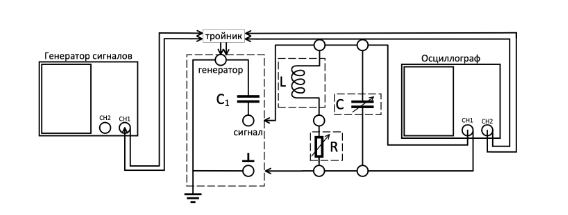
\includegraphics[width=.8\textwidth]{2.png}}
\caption{Схема установки для исследования АЧХ и ФЧХ}
\end{figure}
\end{center}

\par 1) Для наблюдения вынужденных колебаний переведем осциллограф в одноканальный режим просмотра (выключить режим XY). \\

\par 2) Переведем генератор специальных сигналов в режим подачи синусоидального сигнала. \\

\par 3) Выставим ранее найденные значения емкости и сопротивления $C^*$ и $R_1$. \\

\par 4) С помощью переходника и коаксиальных кабелей подадим сигнал с генератора одновременно на колебательный контур и на канал 2 осциллографа. Добъемся того чтобы на экране осциллографа можно было наблюдать одновременно два сигнала: сигнал, взятый с колебательного контура, на первом канале и первоначальный сигнал на втором канале.

\par 5) Убедитимся, что на экране осциллографа при частотах близких к резонансным наблюдается устойчивый синусоидальный сигнал.\\

\par 6) Изменяя частоту генератора вблизи резонансной частоты и наблюдая синусоиду на первом канале на экране осциллографа, убедимся, что амплитуда колебаний максимальна при достижении резонансной частоты. Определим ее значение: $\nu_{\text{рез}} \approx$ 6490 Гц. \\

\par 7) Снимем АЧХ колебательного контура вблизи резонанса. Амплитуда резонансной частоты: $U_{\text{рез}} \approx$ 1.06 В. Повторим измерения для $R_2$, где $\nu_{\text{рез}}$ = 6610 Гц  и $U_{\text{рез}}$ = 604 мВ: \\

\begin{center}
\begin{tabular}{|c|c|c|c|c|c|}
	\hline
	$R_1$, Ом & $\nu_1$, Гц & $U_1$, мВ & $R_2$, Ом & $\nu_2$, Гц & $U_2$, мВ \\
	\hline
	\multirow{22}{*}{816.50 $\pm$ 1.50 Ом} & 2850 & 66 & \multirow{23}{*}{1633.00 $\pm$ 3.00} & 4600 & 244 \\
	\cline{2-3} \cline{5-6} & 3200 & 83 & & 4800 & 284 \\
	\cline{2-3} \cline{5-6} & 3550 & 106 & & 5000 & 316 \\
	\cline{2-3} \cline{5-6} & 3900 & 142 & & 5200 & 356 \\
	\cline{2-3} \cline{5-6} & 4250 & 184 & & 5400 & 396 \\
	\cline{2-3} \cline{5-6} & 4600 & 242 & & 5600 & 444 \\
	\cline{2-3} \cline{5-6} & 4950 & 322 & & 5800 & 492 \\
	\cline{2-3} \cline{5-6} & 5300 & 438 & & 6000 & 532 \\
	\cline{2-3} \cline{5-6} & 5650 & 608 & & 6200 & 572 \\
	\cline{2-3} \cline{5-6} & 6000 & 824 & & 6400 & 592 \\
	\cline{2-3} \cline{5-6} & 6350 & 1010 & & 6600 & 604 \\
	\cline{2-3} \cline{5-6} & 6700 & 1000 & & 6800 & 604 \\
	\cline{2-3} \cline{5-6} & 7050 & 890 & & 7000 & 596 \\
	\cline{2-3} \cline{5-6} & 7400 & 748 & & 7200 & 580 \\
	\cline{2-3} \cline{5-6} & 7750 & 644 & & 7400 & 564 \\
	\cline{2-3} \cline{5-6} & 8100 & 572 & & 7600 & 548 \\
	\cline{2-3} \cline{5-6} & 8450 & 528 & & 7800 & 528 \\
	\cline{2-3} \cline{5-6} & 8800 & 476 & & 8000 & 512 \\
	\cline{2-3} \cline{5-6} & 9150 & 440 & & 8200 & 492 \\
	\cline{2-3} \cline{5-6} & 9500 & 416 & & 8400 & 476 \\
	\cline{2-3} \cline{5-6} & 9850 & 396 & & 8600 & 456 \\
	\cline{2-3} \cline{5-6} & 10200 & 380 & & 8800 & 436 \\
	\cline{2-3} \cline{5-6} & & & & 9000 & 424 \\
	\hline
\end{tabular}
\end{center}

\par Построим на одном графике резонансные кривые в координатах U/$U_0$ = f($\nu$/$\nu_0$), где $U_0$ - напряжение при резонансной частоте $\nu_0$:

\pgfplotstableread{
x			y 			y-max		y-min
0.439		0.0623		0.0005		0
0.493		0.0783		0.0005		0
0.547		0.1000		0.0005		0
0.601		0.1340		0			0
0.655		0.1736		0			0
0.709		0.2283		0			0
0.763		0.3038		0			0
0.817		0.4132		0			0
0.871		0.5736		0			0
0.924		0.7774		0			0
0.978		0.9528		0			0
1.032		0.9434		0			0
1.086		0.8396		0			0
1.140		0.7057		0			0
1.194		0.6075		0			0
1.248		0.5396		0			0
1.302		0.4981		0			0
1.360		0.4491		0			0
1.410		0.4151		0			0
1.464		0.3925		0			0
1.518		0.3736		0			0
1.572		0.3585		0			0
}{\mytable}

\begin{center}
\begin{tikzpicture}
\begin{axis} [
	title = $U/U_0(\nu/\nu_0)$,
	xlabel = {$\nu/\nu_0$},
	ylabel = {$U/U_0$},
	minor tick num = 2,
	grid = major
]

\addplot +[mark options = {scale = 0.1,}]
	plot [error bars/.cd, y dir=both, y explicit]
	table [y error plus=y-max, y error minus=y-min] {\mytable};

\pgfplotstableread{
x			y		y-max	y-min
0.696		0.4040	0		0
0.726		0.4702	0		0
0.756		0.5232	0		0
0.787		0.5894	0		0
0.817		0.6556	0		0
0.847		0.7351	0		0
0.877		0.8146	0		0
0.908		0.8808	0		0
0.938		0.9470	0		0
0.968		0.9801	0		0
0.998		1		0		0
1.029		1		0		0
1.059		0.9868	0		0
1.089		0.9603	0		0
1.120		0.9338	0		0
1.150		0.9073	0		0
1.180		0.8742	0		0
1.210		0.8477	0		0
1.241		0.8146	0		0
1.271		0.7881	0		0
1.301		0.7550	0		0
1.331		0.7219	0		0
1.362		0.7020	0		0
}{\mytable}	

\addplot +[mark options = {scale = 0.1}] 
	plot [error bars/.cd, y dir=both, y explicit]
	table [y error plus=y-max, y error minus=y-min] {\mytable};
\end{axis}
\end{tikzpicture}
\end{center}

\par Определим добротность контура по формуле Q = $\omega_0/2\Delta\Omega$, где 2$\Delta\Omega$ - ширина резонансной кривой, измеренная на уровне f(1)/$sqrt(2)$

\begin{center}
\begin{tabular}{|c|c|}
	\hline
	$R_1$ = (816.50 $\pm$ 1.50) Ом & $Q_1$ = \\
	\hline
	$R_2$ = (1633.00 $\pm$ 3.00) Ом & $Q_2$ = \\ 
	\hline
\end{tabular}
\end{center}

\par \textbf{Процессы установления и затухания} 

\begin{figure}
\center{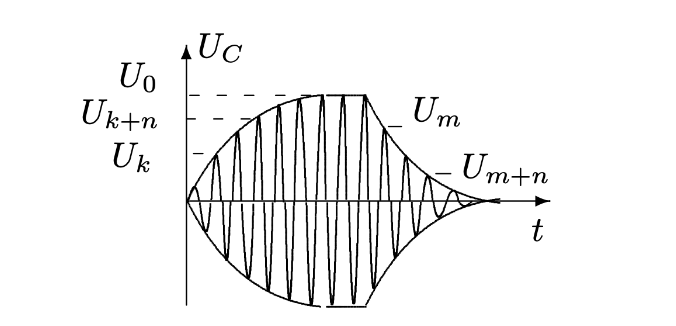
\includegraphics[width=.8\textwidth]{3.png}}
\caption{Нарастание и затухание вынужденных колебаний}
\end{figure}



\end{document}
